\documentclass[11pt,a4paper]{article}

\usepackage[T1]{fontenc}
\usepackage[utf8]{inputenc}
\usepackage{lmodern}
\usepackage[margin=2.1cm]{geometry}
\usepackage{amsmath,amssymb}
\usepackage{booktabs}
\usepackage{graphicx}
\usepackage{caption}
\usepackage{enumitem}
\usepackage{xcolor}
\usepackage[colorlinks=true,linkcolor=black,citecolor=black,urlcolor=blue]{hyperref}

\graphicspath{{fig/}{../fig/}}
\captionsetup{font=small,labelfont=bf}
\setlist{nosep,leftmargin=1.4em}
\definecolor{soft}{RGB}{244,242,238}
\newcommand{\thc}{\theta_c}
\newcommand{\dtr}{\Delta_{\mathrm{tr}}}
\newcommand{\sdl}[1]{\operatorname{sd}(\ln #1)}

\title{\textbf{Residual PCC capacity in severe propionic acidaemia:\\
what the clinical record identifies, and what the dosing interval needs}}
\author{Guido Putignano}
\date{Technical note, November 2026}

\begin{document}
\maketitle

\noindent\colorbox{soft}{\parbox{\dimexpr\linewidth-2\fboxsep}{\small
\textbf{Summary.} The paper shows that the fortnightly dose train identifies residual
capacity $\theta$ at the illustrative patient, $\sdl{\hat\theta}=0.17$ from 25 monthly draws
at normal capacity. This note asks the same question where it matters clinically, in
severe propionic acidaemia at $5\%$ of normal, and reports four results.
\begin{enumerate}[leftmargin=1.5em,topsep=3pt]
\item \textbf{Absolute capacity is not practically identifiable at $5\%$.} The same record
gives $\sdl{\hat\theta}=3.07$ against a target of $0.20$. The cause is structural: at low
capacity every steady-state draw constrains $\theta$ and the alternative clearance $k_e$
along almost the same direction ($\operatorname{corr}=-0.99$), and $k_e$ carries $98\%$ of
the variance.
\item \textbf{No available instrument closes the gap.} An observable fixes $\theta$ either
through the mass balance, which needs the shape of the competing clearance, or by direct
transduction, which needs a calibration constant. None of these constants is measured in
humans. The best combination of real sensors reaches $0.44$.
\item \textbf{Change within one patient is identifiable in the model} ($0.13$ between two
windows of weekly draws), because every unknown patient constant cancels in the contrast.
Whether it holds in patients depends on the marker's within-patient variability in PA,
which is unmeasured.
\item \textbf{The dosing interval does not need $\theta$; it needs the PCC protein
half-life.} The interval is safe for every patient when the drug's trough increment exceeds
the critical capacity. Under the parent model this holds at 14 and 15 days for half-lives
above $2.6$--$3.2$\,d. The 21-day interval turns on the half-life: the crossing is
$3.55$\,d at the nominal constants, the only human measurement is $3.6$\,d, and the liver
value, which is the one that matters, is unmeasured (estimate $4.3$\,d).
\end{enumerate}
\vspace{-2pt}
All records are simulated on the paper's illustrative constants; no patient data are used.
}}

\vspace{0.6em}
\begin{table}[h]
\centering\small
\caption{\label{tab:key}Key numbers at $5\%$ of normal capacity. Precision is the
Cram\'er--Rao bound on the log scale; the target is $0.20$ (about $\pm20\%$).}
\begin{tabular}{@{}lll@{}}
\toprule
quantity & value & condition \\
\midrule
$\sdl{\hat\theta}$, 25 monthly draws & $3.07$ & paper's design; $0.17$ at normal capacity \\
\quad $+$ both tracers ($k_e$ and load) & $0.44$ & best real sensor combination \\
\quad load and $k_e$ known exactly & $0.29$ & idealised floor \\
$\sdl{\hat\theta_2}-\ln\hat\theta_1$, within patient & $0.13$ & $2\times104$ weekly draws,
$5\%$ per-draw CV \\
\quad at the measured serial CV & $0.475$ & $26.4\%$ per-draw CV (healthy adults) \\
$\sdl{\lambda}$, drug-increment decay rate & $0.055$ & 2 years of monthly draws \\
21-day crossing (PCC half-life) & $3.545$\,d & nominal carnitine constants \\
\quad over the admissible constants & $3.29$--$4.08$\,d & corners of the parent model's box \\
human PCC half-life & $3.6$\,d & fibroblast; liver unmeasured, estimate $4.3$\,d \\
\bottomrule
\end{tabular}
\end{table}

\section{Setting}

The marker obeys the paper's parent balance,
\begin{equation}
\dot m = L(t) + L_0 - \bigl(\theta+\Delta(t)\bigr)g(m) - \alpha(m),\qquad
g(m)=\frac{m}{K_m+m},
\label{eq:parent}
\end{equation}
with $\alpha$ the carnitine-conjugation channel. Identifiability is computed on the local
identification model, $\alpha(m)\to k_e m$; the dosing decision uses the parent model's
intrinsic critical capacity. The footing is the paper's: normal capacity $\theta=3000$\,\textmu
M/d (so $5\%$ is $\theta=150$), $K_m=100$\,\textmu M, $k_e=5$\,d$^{-1}$; 25 monthly draws over
two years on the fortnightly dose train (amplitude $6000$\,\textmu M/d, assumed increment
half-life $3.5$\,d); recorded load with $10\%$ day-to-day variation, a $5\%$ prior on the
unrecorded load, a $5\%$ assay CV and a prior of $0.8$ on $\ln k_e$. Log-scale precisions are
read from the Fisher information; one-sided decisions (threshold crossings, margins) are
checked by simulation, because the posterior at $5\%$ is strongly log-normal and first-order
propagation of it is unreliable.

\section{Result 1: absolute capacity at 5\% of normal}

Figure~\ref{fig:t1}(a) shows the precision of the paper's design across the disease range.
It meets the target only between $82\%$ and $627\%$ of normal, with its best value
($0.123$) at $212\%$; it is $3.07$ at $5\%$ and $14.75$ at $1\%$. The reason is in
panel~(b): below about $50\%$ of normal, $\ln\theta$ is almost perfectly confounded with
$\ln k_e$. At $5\%$ the enzyme carries only about $16\%$ of the load, so a steady-state draw
cannot tell a larger $\theta$ from a smaller $k_e$. Even with $k_e$ known exactly a residual
$0.39$ remains at 25 draws (the load record contributes $62\%$ of it, the assay $29\%$); it
then falls as $1/\sqrt n$ and crosses $0.20$ near 300 draws. At the precision a safe
transient can deliver on $k_e$ (about $0.2$ on the log scale) no sampling rate reaches even
$0.30$. The profile likelihood (panel~c) is flat towards zero: the record supports a one-sided
statement, $\theta$ below about $22\%$ of normal at the $95\%$ level, not a point estimate.

\begin{figure}[t]
\centering
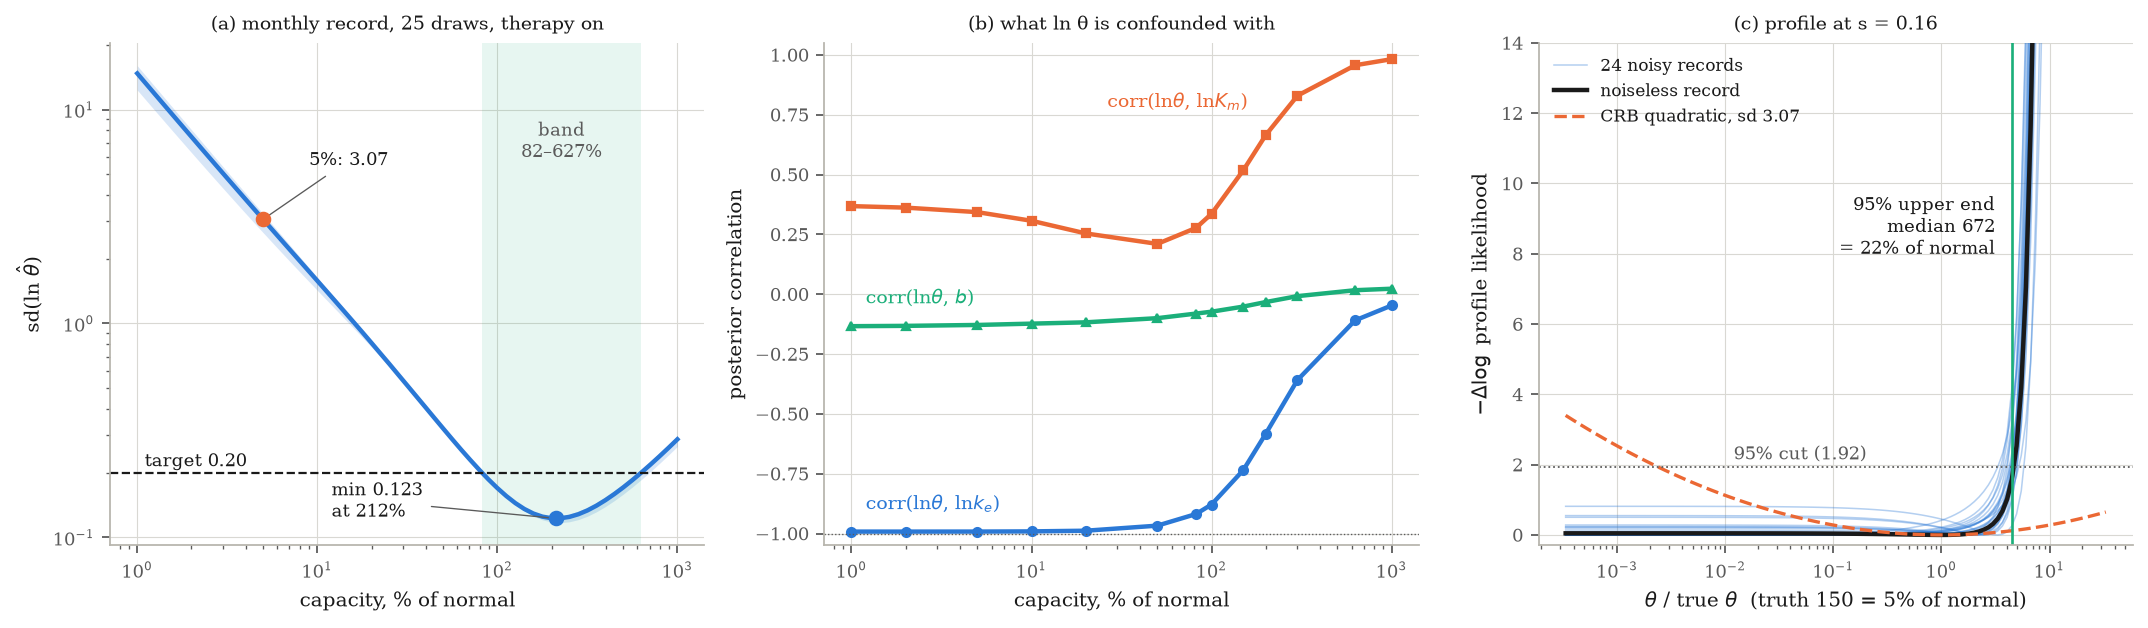
\includegraphics[width=\linewidth]{t1_identifiability.png}
\caption{\label{fig:t1}(a) $\sdl{\hat\theta}$ of the paper's design (25 monthly draws,
therapy on) against residual capacity; the target $0.20$ is met only in the shaded band.
(b) Posterior correlation of $\ln\theta$ with $\ln k_e$, $\ln K_m$ and the load bias $b$.
(c) Profile likelihood at $5\%$ of normal for 24 simulated records and the noiseless record,
against the quadratic (Cram\'er--Rao) approximation.}
\end{figure}

\paragraph{The same result as geometry.} At steady state, moving the known increment to the
right-hand side turns each draw into a line in the $(\theta,k_e)$ plane,
\begin{equation}
g(m_i)\,\theta + m_i\,k_e = L_i - \Delta_i\,g(m_i),
\qquad \text{slope } \frac{dk_e}{d\theta}=-\frac{1}{K_m+m_i}.
\label{eq:pencil}
\end{equation}
Noise-free and at the true $K_m$ the lines are concurrent at the true $(\theta,k_e)$. Over the
dosed record's band ($m\approx4$--$38$\,\textmu M) every slope lies between $-0.0096$ and
$-0.0074$, so the pencil is nearly parallel (Fig.~\ref{fig:pencil}a). Its weighted
concurrence region has correlation $-0.998$ and aspect ratio $29{:}1$, and it coincides with
the inverse Fisher information at fixed $K_m$; letting $K_m$ vary slides the concurrence
point along the fibre, and the two together give the headline $3.07$. The $300$ pairwise
intersections scatter like a Cauchy sample (only $5\%$ fall within a factor of three of the
truth), so on the natural scale the record has no usable point estimate, only a log-scale
width. A wide load excursion fans the slopes and the intersections concentrate
(Fig.~\ref{fig:pencil}b, $41\%$ within a factor of three), but an excursion of that width
exceeds the parent model's crisis threshold of $1.177$ times the baseline load, so it is
not an admissible experiment. The residual distances of the lines to their best common point
also give a calibrated test of model adequacy: it detects a mis-recorded load, but not a
second saturable clearance channel, which is nearly collinear with $\{g(m),m\}$ over any
realistic band and is absorbed along the fibre.

\begin{figure}[t]
\centering
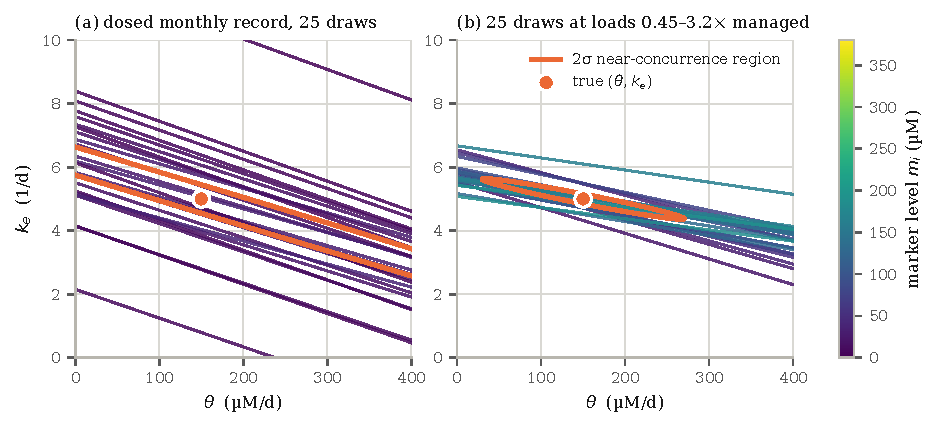
\includegraphics[width=\linewidth]{pi_pencil.pdf}
\caption{\label{fig:pencil}Each steady-state draw as a line \eqref{eq:pencil} in the
$(\theta,k_e)$ plane, coloured by the marker level. (a) The dosed monthly record: all slopes
are close to $-1/K_m$, the lines are nearly parallel and the $2\sigma$ near-concurrence
region is a long sliver. (b) A record with one wide load excursion: the high-marker draws
change the slope and the region closes, at a load the parent model does not tolerate.}
\end{figure}

\section{Result 2: no available instrument closes the gap}

Figure~\ref{fig:routes} collects every route to absolute $\theta$ at $5\%$. Measuring the
nuisances does not suffice: an isotope-dilution load turnover adds almost nothing ($3.04$),
an intravenous $^{13}$C$_3$ tracer for $k_e$ at $5.4\%$ brings the record to $0.45$, both
together to $0.44$, and even exact knowledge of both leaves $0.29$. $k_e$, not the load, is
the binding nuisance. Only readings of the enzyme itself reach $0.20$, and each needs a
calibration constant that is not available. An ex vivo PCC assay at its $20\%$
repeatability reaches $0.20$ if the scale factor from cell activity to whole-body capacity is
known, and reverts to $3.05$ if it is not. Expressing the assay as a ratio to healthy controls
cancels the population scale factor, but then it measures in vitro activity; read as the
whole-body capacity in \eqref{eq:parent}, it carries a per-patient mapping error that does not
cancel, about $0.65$ at the only same-subject data (in methylmalonic acidaemia, $R^2=0.33$;
Manoli et al., 2021). A calibrated in vivo flux reading $O=c\,\theta g(m)$ reaches the target
if $\sqrt{Y^2+Z^2}\lesssim19\%$, with $Y$ the reading precision and $Z$ the uncertainty of the
recovery $c$; the $^{13}$C-propionate breath test does not meet this, since its recovery is
not calibrated per subject and its within-subject CV in the one repeated-test series is
$14\pm13\%$.

\begin{figure}[t]
\centering
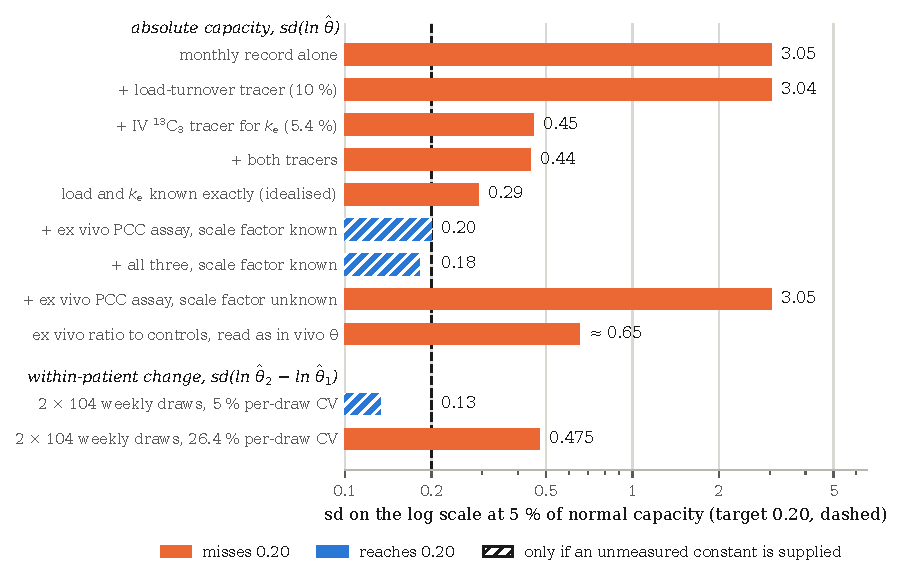
\includegraphics[width=0.86\linewidth]{pi_routes.pdf}
\caption{\label{fig:routes}Every route to $\theta$ at $5\%$ of normal on one log scale.
Upper group: absolute capacity (the record-alone value $3.05$ is the same record evaluated in
the joint multi-sensor model). Hatched bars reach $0.20$ only when an unmeasured calibration
is supplied. Lower group: change between two windows, a different quantity, at two values of
the per-draw marker variability.}
\end{figure}

The pattern is structural. $\theta$ enters the model only as the maximal velocity of the
flux $\theta g(m)$, so an observable depends on it in one of two ways. Either it depends on
the states $\theta$ helps set, and inverting the balance requires the shape of the competing
channel ($k_e$ in the local model, its half-saturation $K_e$ in the saturating variant, and
the carnitine constants $K_c$, $M_i$, $\rho_0$, $R_0$ in the parent model); or it reads the
flux directly, and requires a transduction constant. A marker of an upstream pool (C3,
2-methylcitrate) needs both. The parent model is the decisive check, because there the
competing channel has its own observable, free carnitine: with the channel constants free the
precision is about $16$ (about $20$ without the carnitine reading), and with them known it is
$0.34$, a value the marker alone already reaches once the constants are known. Observing the
competing channel does not remove the need to know its shape.

The magnitude, though not the sign, depends on the clearance structure. The local model's
linear clearance gives the alternative route about $84\%$ of the load at $5\%$ capacity,
which is high against the PA literature, where measured urinary output of propionate
metabolites is a few per cent of estimated production (Thompson et al., 1990). Under the
saturating-clearance variant, at a constructed point consistent with that literature, the
enzyme's share is larger and the precision is $0.29$ ($0.92$ at the variant's nominal
constants, which never decompensate); the target is touched ($\approx0.19$) only at a low
clearance ceiling with $K_e$ assumed known to about $30\%$.

\section{Result 3: change within one patient}

The contrast $\ln\hat\theta_2-\ln\hat\theta_1$ between two windows is a different estimand,
and every patient constant that blocks the absolute level ($k_e$, the load bias, $K_m$, any
assay scale factor) is common to both windows and cancels. Two windows of 104 weekly draws
give $\operatorname{sd}=0.13$, enough to detect a $+45\%$ rise or a $-30\%$ fall with $80\%$
power; the precision depends on draws per window, not on calendar span. This is a model
floor with two conditions. First, it assumes a $5\%$ per-draw marker variability; at the only
published serial within-subject CV for plasma C3, $26.4\%$ in healthy adults, it becomes
$0.475$ and would need about 590 draws per window, so the result holds only if the
within-patient variability in PA is below about $10\%$, which has not been measured. Second,
the patient constants must actually be constant: a drift of $0.06$ in $\ln k_e$ between
windows already gives $0.28$. The load is the critical case. Gut-derived propionate is
antibiotic-suppressible (Thompson et al., 1990, metronidazole), and an unrecorded antibiotic
course between windows fakes an apparent capacity rise of $1$ to $3$ log units, in the
direction of reassurance. Antibiotic status should therefore be recorded with the load.

\section{Result 4: what the dosing interval needs}

The interval decision is a trough condition. With the same delivered rate at every interval
$\tau$, the increment's trough is
\begin{equation}
\dtr(\tau) = D\,\frac{\tau}{14}\,\frac{e^{-\lambda\tau}}{1-e^{-\lambda\tau}},\qquad
\lambda=\frac{\ln 2}{t_{1/2}},
\end{equation}
and the interval is safe while $\theta+\dtr(\tau)>\thc$. The parent model's intrinsic
critical capacity at baseline load is $\thc=150.8$\,\textmu M/d, essentially the $5\%$
patient's own capacity. At the design's half-life of $3.5$\,d, $\dtr(14)=400$\,\textmu M/d,
so the fortnightly interval is safe for every residual capacity, including $\theta=0$. The
decision therefore does not depend on $\theta$ at all; it depends on $t_{1/2}$, the decay
rate of the delivered enzyme. Figure~\ref{fig:margin} plots the margin of a patient with no
residual capacity, $\mu(\tau)=\dtr(\tau)-\thc$. It is positive for half-lives above
$2.62$\,d at 14 days, $2.75$\,d at 15 days and $3.545$\,d at 21 days.

\begin{figure}[t]
\centering
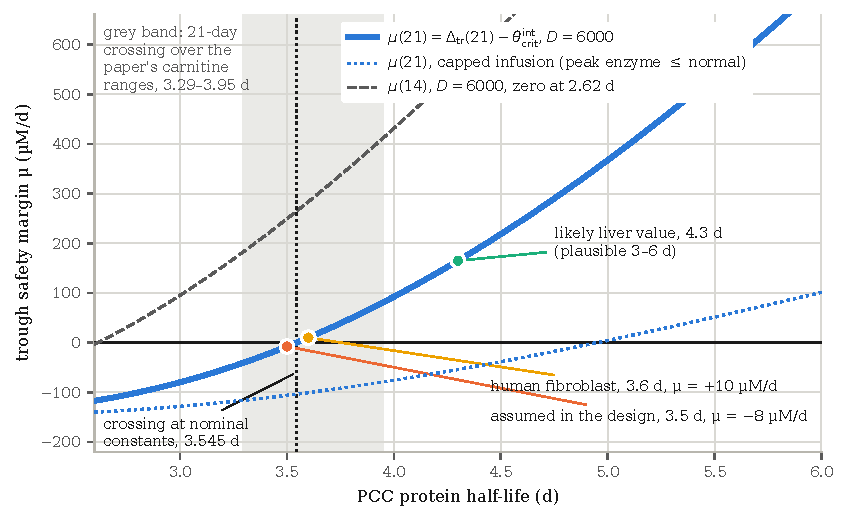
\includegraphics[width=0.84\linewidth]{pi_margin.pdf}
\caption{\label{fig:margin}Trough safety margin of a patient with no residual capacity,
$\mu=\dtr-\thc$, against the PCC protein half-life, at the parent model's nominal carnitine
constants ($K_c=100$). Right of the crossing the 21-day interval is safe for every patient
without knowing $\theta$; left of it the decision needs $\theta$. The grey band is the range
of the 21-day crossing over the corners of the admissible carnitine constants.}
\end{figure}

The only human measurement of PCC turnover, in fibroblasts (Chandler \& Ballard, 1985), is
$3.6$\,d: $1.5\%$ above the 21-day crossing, a margin of $+10$\,\textmu M/d, while the
design's assumed $3.5$\,d sits just below it ($-8$\,\textmu M/d). The relevant value is the
liver's, which has not been measured. PCC is a mitochondrial-matrix enzyme, and the median
turnover of mouse liver mitochondrial proteins is $4.26$\,d (Kim et al., 2012), which places
hepatic PCC at about $4.3$\,d, plausibly $3$--$6$\,d. On that band the probability that the
liver half-life lies above the crossing is about $64$--$71\%$, a rough guide rather than a
measured probability.

Two qualifications bound this result.

\emph{The crossing depends on unmeasured constants.} $\thc$ depends on the carnitine
channel's $K_c$, $M_i$ and $\rho_0$, none of which is measured. Over the corners of the
admissible box the 21-day crossing moves from $3.29$ to $4.08$\,d (Fig.~\ref{fig:margin}):
$3.6$\,d clears it at six of the eight corners and fails, for example, at $K_c\le50$, while
$4.3$\,d clears it everywhere. The 14- and 15-day floors rise to at most $3.06$ and $3.21$\,d,
so the 14- and 15-day conclusions hold whenever the liver half-life exceeds about $3.2$\,d.
At the least favourable constants the probability above falls to $54$--$59\%$.

\emph{What the record can resolve.} The on-therapy record identifies $\lambda$ itself:
$\sdl{\lambda}=0.055$ after two years of monthly draws ($\pm25\%$ within six months, $\pm5\%$
within one to four years), and it separates a $3.6$\,d from a $7$\,d half-life at $7\sigma$
within six months. Placing a value on one side of the crossing is a much finer question
(Table~\ref{tab:lambda}). If the true value is near $3.6$\,d, no single patient's record does
it at any length; a pooled estimate would need $23$ to $155$ patients, depending on cadence,
record length and power, and only if $\lambda$ is common to all of them. If it is near
$4.3$\,d, one record places it with $80\%$ probability within a year of monthly draws against
the nominal crossing, but not against the highest crossing in the box. Estimating $\theta$
from the passive record does not rescue the 21-day interval when the half-life is below the
crossing: by simulation, the margin estimate stays about $\pm140$\,\textmu M/d wide from six
months to five years.

\begin{table}[t]
\centering\small
\caption{\label{tab:lambda}Separation of two half-life hypotheses by one patient's record,
in units of the record's $\sdl{\lambda}$ evaluated at the true value; in brackets, the
probability that one record clears $2\sigma$, $\Phi(z-2)$. These are Fisher-information
values and have not been checked by simulation.}
\begin{tabular}{@{}lcccc@{}}
\toprule
record & $3.6$ vs $7$\,d & $3.6$\,d vs crossing & $4.3$\,d vs $3.545$\,d & $4.3$\,d vs $4.08$\,d \\
\midrule
6 months, monthly  & $7.0$  & $0.16$ & $1.93$ ($47\%$) & $0.52$ ($7\%$) \\
12 months, monthly & $9.9$  & $0.23$ & $2.97$ ($83\%$) & $0.80$ ($11\%$) \\
6 months, weekly   & $12.5$ & $0.29$ & $3.71$ ($96\%$) & $1.00$ ($16\%$) \\
5 years, weekly    & $25.0$ & $0.58$ & $7.22$ ($>99\%$) & $1.94$ ($47\%$) \\
\bottomrule
\end{tabular}
\end{table}

\section{Limitations}

\begin{itemize}
\item Every record is simulated, for one illustrative patient on the paper's illustrative
constants. Absolute precisions depend on those constants; the structural statements
(the confounding, the two ways an observable reaches $\theta$, the cancellation in the
contrast) do not.
\item The identifiability results are computed on the local identification model, whose
linear clearance is not the PA phenotype. They were rechecked under the saturating variant
(at its nominal constants, at a constructed point and over a grid) and under the parent model
(at its nominal constants and over its channel constants), and the cross-sectional verdict
kept its sign. The identifiability under a bounded clearance calibrated to the literature,
with the crisis boundary treated explicitly, has not been done. The within-patient contrast
was rechecked under the saturating variant ($0.088$) but not under the parent model.
\item The model has no propionyl-CoA state, so the C3 and 2-methylcitrate markers are not
represented.
\item The dosing results use the parent model's intrinsic critical capacity, which depends on
the unmeasured carnitine constants (Result~4), and the human liver half-life, which is
unmeasured.
\end{itemize}

\section{What would settle the open points}

\begin{enumerate}
\item \textbf{The hepatic PCC half-life.} It is contained in the mRNA-3927 trial's on-therapy
marker record (NCT04159103) and in the sponsor's population pharmacokinetic model (Gao et
al., ACoP 2025), neither of which is public. Either would settle the 14- and 15-day
intervals outright and the 21-day interval unless the value lies within the crossing's range.
\item \textbf{The marker's within-patient variability in PA.} Serial C3 and 2-methylcitrate
values, or their within-patient CV, would decide whether within-patient monitoring is
deliverable. A request has been made to the authors of the 2020 decompensation-phenotyping
study (Haijes et al., 2020); no reply yet.
\item \textbf{Antibiotic status in the load record}, at no cost, as a precondition for any
within-patient comparison.
\item \textbf{A paired ex vivo and in vivo study in PA} (fibroblast PCC activity and the
$^{13}$C-propionate breath test in the same patients), which would measure the mapping that
the ratio route currently has to borrow from methylmalonic acidaemia.
\end{enumerate}

\section*{References}
{\small
\begin{itemize}[leftmargin=1em,label={}]
\item Chandler \& Ballard (1985). Turnover of propionyl-CoA carboxylase in human fibroblasts,
$[^3$H$]$biotin pulse--chase.
\item Haijes, H.\,A., Jans, J.\,J.\,M., van der Ham, M., van Hasselt, P.\,M., Verhoeven-Duif,
N.\,M. (2020). Understanding acute metabolic decompensation in propionic and methylmalonic
acidemias: a deep metabolic phenotyping approach. \emph{Orphanet J.\ Rare Dis.} 15:68.
\item Kim et al.\ (2012). Turnover of the mouse liver mitochondrial proteome, metabolic
labelling.
\item Manoli, I., Pass, A.\,R., Harrington, E.\,A., et al.\ (2021). 1-$^{13}$C-propionate
breath testing as a surrogate endpoint to assess efficacy of liver-directed therapies in
methylmalonic acidemia (MMA). \emph{Genet.\ Med.} 23(8).
\item Thompson, G.\,N., Walter, J.\,H., Bresson, J.-L., et al.\ (1990). Sources of propionate
in inborn errors of propionate metabolism. \emph{Metabolism} 39(11):1133--1137.
\item Thompson, G.\,N., Chalmers, R.\,A., Walter, J.\,H., et al.\ (1990). The use of
metronidazole in management of methylmalonic and propionic acidaemias. \emph{Eur.\ J.\
Pediatr.} 149(11):792--796.
\end{itemize}}

\end{document}
